%==============================================================================
% presentation.tex
%==============================================================================


%==============================================================================
% Configuration
%==============================================================================

% Internationalisation
\usepackage[utf8]{inputenc}
\usepackage[T1]{fontenc}
% \usepackage[ngerman]{babel}

% Different packages
\usepackage{url}
\usepackage{color,listings,paralist}
\usepackage{enumerate}
\usepackage{tabularx}
\usepackage{alltt}

% Use default Acrobat reader fonts
\usepackage{mathpazo}

% Use CM fonts (increases document size)
\usepackage{ae}

% Use images
\usepackage{graphicx}

% Configure beamer
\usetheme[secheader]{Ikhono}
\usefonttheme[onlylarge]{structurebold}
\setbeamertemplate{navigation symbols}{}

% Variables
\providecommand{\Title}{Parallel Programming}
\providecommand{\Subtitle}{Recitation Session 12}
\providecommand{\Author}{Thomas Weibel <weibelt@ethz.ch>}
\providecommand{\Institute}{Laboratory for Software Technology, \\
  Swiss Federal Institute of Technology Z\"urich}
\providecommand{\Date}{June 3, 2010}

% PDF settings
\hypersetup{
  pdftitle={\Title, \Subtitle},
  pdfauthor={\Author},
  pdfsubject={\Institute},
  pdfkeywords={parallel programming} 
}

% Titlepage
\title{\Title}
\subtitle{\Subtitle}
\author{\Author}
\institute{\Institute}
\date{\Date}

% Listings
\lstdefinestyle{Default}{
  language=Java,
  tabsize=2,
  mathescape=true,
  inputencoding=utf8,
  showstringspaces=false,
  fontadjust=true,
  basicstyle=\ttfamily,
  keywordstyle=\color{blue}\bfseries,
}
\lstset{style=Default}


%==============================================================================
% Document
%==============================================================================

\begin{document}


% Titlepage
\begin{frame}[plain]
  \titlepage
\end{frame}


\section*{Introduction}

\begin{frame}{Executive Summary}
  \begin{itemize}
  \item Linearizability
  \item Assignment 11
    \begin{itemize}
    \item Proving program properties
    \item Possible executions
    \end{itemize}
  \end{itemize}

  \vspace{\stretch{1}}

  \begin{center}
    \includegraphics[scale=0.4]{figures/dilbert-iit}
  \end{center}
\end{frame}


\section{Linearizability}

\begin{frame}{Outline}
  \tableofcontents[current]
\end{frame}

\begin{frame}{Definition}
  \begin{itemize}
  \item Each method should
    \begin{itemize}
    \item ``take effect''
    \item Instantaneously
    \item Between invocation and response events
    \end{itemize}
  \item Object is correct if this ``sequential'' behavior is correct
  \item Any such concurrent object is \alert{Linearizable}
  \end{itemize}
\end{frame}

\begin{frame}{Is it really about the object?}
  \begin{itemize}
  \item Each method should
    \begin{itemize}
    \item ``take effect''
    \item Instantaneously
    \item Between invocation and response events
    \end{itemize}
  \item Observation: methods must appear to execute in a one-at-a-time
    sequential order
  \item Sounds like a property of an execution
  \item A linearizable object: one all of whose possible executions
    are linearizable
  \end{itemize}
\end{frame}

\begin{frame}{Linearizability in Practice}
  \begin{thebibliography}{10}
    \beamertemplatearticlebibitems
    
  \bibitem{linearizability}
    Herlihy and Shavit, {\em The Art of Multiprocessor Programming}, Chapter 3
    \url{www.elsevierdirect.com/companions/9780123705914}

  \bibitem{deque}
    Hendler, et al., {\em A Dynamic-sized Nonblocking Work Stealing Deque},
    \url{www.springerlink.com/index/Y7HQ174L92170355.pdf}

  \bibitem{concurrent-queues}
    Michael and Scott, {\em Simple, Fast, and Practical Non-blocking and Blocking Concurrent Queue Algorithms},
    \url{portal.acm.org/citation.cfm?id=248052.248106}
  \end{thebibliography}  
\end{frame}


\section{Proving Program Properties}

\begin{frame}{Outline}
  \tableofcontents[current]
\end{frame}

\begin{frame}{Variant of Peterson's Solution}
  \begin{columns}[c]
    \begin{column}{0.35\textwidth}
      \begin{itemize}
      \item Proving that this variant of Peterson's solution works
      \item Equivalent to question 2 of the example exam
      \item See lecture of June 1st, 2010
      \end{itemize}
    \end{column}
    \begin{column}{0.65\textwidth}
      \begin{center}
        
\includegraphics[width=\textwidth]{figures/dilbert}
      \end{center}
    \end{column}
  \end{columns}
\end{frame}

% \begin{frame}[fragile]{Informal Proof: Example Exam, Question 2}
%   \begin{itemize}
%   \item Shared variables are volatile, hence inter-thread
%     communication is ensured
%   \item Each thread writes it's own flag
%   \end{itemize}

%   \vspace{\stretch{1}}

%   1) Initial Condition:

%   \begin{lstlisting}
% flag0 = false;
% flag1 = false;
% victim = 0;    
%   \end{lstlisting}
% \end{frame}

% \begin{frame}[fragile]{Informal Proof: Example Exam, Question 2}
%   2) State before critical section:

%   \begin{lstlisting}
% Thread0: 
%   flag0 = true, victim = 0 || 1, 
%   no write to flag1; (line 12)

% Thread1: 
%   flag1 = true, victim = 0 || 1, 
%   no write to flag0; (line 27)
%   \end{lstlisting}
% \end{frame}

% \begin{frame}[fragile]{Informal Proof: Example Exam, Question 2}
%   3) Invariants:

%   \begin{lstlisting}
% 3a) Thread 0: 
%       flag1 = false || victim = 1; 
%       (line 12 -> line 13)

% 3b) Thread 1: 
%       flag0 = false || victim = 0; 
%       (line 27 -> line 28)

% 3c) Thread 0 and Thread 1 at line 13 
%     and line 28 at the same time
%   \end{lstlisting}

%   To enter the critial section, thead 0 must transition from line 12
%   to line 13, thread 1 must transition from line 27 to 28. So we only
%   need to consider the case when both threads are in the while and
%   therefore \lstinline!flag0! and \lstinline!flag1! are true.
% \end{frame}

% \begin{frame}[fragile]{Informal Proof: Example Exam, Question 2}
%   4) Proof: Thread 0 in CS, thread 1 wants to enter

%   \begin{lstlisting}
% flag0 = true (line 10); 
% flag1 = true;
% victim = 1 (line 26);

% => 3b) does not evaluate to true
%   \end{lstlisting}

%   \vspace{\stretch{1}}

%   5) Proof: Thread 1 in CS, thread 0 wants to enter

%   \begin{lstlisting}
% flag0 = true (line 25); 
% flag1 = true;
% victim = 0 (line 11);

% => 3a) does not evaluate to true
%   \end{lstlisting}
% \end{frame}

% \begin{frame}{Informal Proof: Example Exam, Question 2}
%   6) Proof: Not both threads in critical section together \\[2ex]

%   If thread 0 and thread 1 were in the CS at the same time, the
%   conditions in 4) and 5) would require that \lstinline!victim! is 0
%   and 1 at the same time\\[3ex]

%   $\rightarrow$ Contradiction
% \end{frame}


\section{Possible Executions}

\begin{frame}{Outline}
  \tableofcontents[current]
\end{frame}

\begin{frame}[fragile]{\lstinline{0 1 2}}
  \begin{columns}[t]
    \begin{column}{0.5\textwidth}
  \begin{lstlisting}
1) T0:
  read f, eval 
  print f

2) T1: 
  read f
  f++
  store f

3) T0: 
  read f, eval
  print f
  read f, eval
  \end{lstlisting}
    \end{column}
    \begin{column}{0.5\textwidth}
  \begin{lstlisting}
4) T1:
  read f
  f++
  store f

5) T0:
  print f
  \end{lstlisting}
    \end{column}
  \end{columns}
\end{frame}

\begin{frame}[fragile]{\lstinline{0 0 2}}
  \begin{columns}[t]
    \begin{column}{0.5\textwidth}
  \begin{lstlisting}
1) T0:
  read f, eval 
  print f
  read f, eval
  print f

2) T1: 
  read f
  f++
  store f

3) T0: 
  read f, eval
  \end{lstlisting}
    \end{column}
    \begin{column}{0.5\textwidth}
  \begin{lstlisting}
4) T1:
  read f
  f++
  store f

5) T0:
  print f
  \end{lstlisting}
    \end{column}
  \end{columns}
\end{frame}

\begin{frame}[fragile]{\lstinline{0 1}}
  \begin{columns}[t]
    \begin{column}{0.5\textwidth}
  \begin{lstlisting}
1) T0:
  read f, eval 
  print f

2) T1: 
  read f
  f++
  store f

3) T0: 
  read f, eval
  print f
  \end{lstlisting}
    \end{column}
    \begin{column}{0.5\textwidth}
  \begin{lstlisting}
4) T1:
  read f
  f++
  store f

5) T0:
  read f, eval
  \end{lstlisting}

  The value 2 will not always appear.
    \end{column}
  \end{columns}
\end{frame}


\section*{Outro}

\begin{frame}{The End}
  \begin{center}
    \huge{Enjoy your ``vacations'' and best of luck for the exam!}
  \end{center}

  \vspace{\stretch{1}}

  \begin{center}
    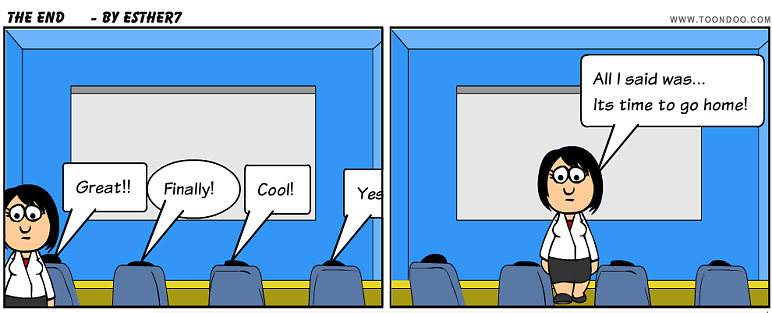
\includegraphics[scale=0.3]{figures/the-end}
  \end{center}
\end{frame}

\end{document}
